This chapter first discusses the experiments carried out in order to both improve the performance, and gain a better understanding, of the sub-components implemented. Experiments such as hyperparameter optimisation and ablation studies including both the two dimensional and three dimensional models are discussed. Once the results are cross-validated, the final results achieved by the optimised models resulting from the experimentation are then presented, interpreted, and compared to results achieved by alternative models. Finally, various aspects of the project are critically evaluated.

\section{Two Dimensional Experimentation}

This section reintroduces the initial results achieved by the ``baseline'' 2D model implemented in Chapter \ref{chap:implementation} and then outlines the experiments carried out in an attempt to improve the performance both qualitatively and quantitatively.

\subsection{Initial Results}

\begin{figure}[!b]
    \begin{subfigure}[b]{0.49\textwidth}
        \centering
        \begin{tikzpicture}[scale=0.9]
            \begin{axis}[
                height=\axisdefaultheight,
                ylabel=\small{Loss},
                xlabel=\small{Epochs},
                grid=major,
                legend pos=north east,
                legend cell align=left,
                legend style={fill=white, fill opacity=0.8, draw=none,text opacity=1}]
                \addplot[blue, mark=x] table [x=xs, y=tl, col sep=comma] {csv/base.csv};
                \addlegendentry{\small{Train Loss}}
                \addplot[magenta, mark=x] table [x=xs, y=vl, col sep=comma] {csv/base.csv};
                \addlegendentry{\small{Val Loss}}
            \end{axis}
        \end{tikzpicture}
        \caption{Loss curve}
    \end{subfigure}
    \hfill
    \begin{subfigure}[b]{0.49\textwidth}
        \centering
        \begin{tikzpicture}[scale=0.9]
            \begin{axis}[
                height=\axisdefaultheight,
                ylabel=\small{Accuracy (pixels)},
                xlabel=\small{Epochs},
                grid=major,
                legend pos=north east,
                legend cell align=left,
                legend style={fill=white, fill opacity=0.8, draw=none,text opacity=1}]
                \addplot[blue, mark=x] table [x=xs, y=ta, col sep=comma] {csv/base.csv};
                \addlegendentry{\small{Train Accuracy}}
                \addplot[magenta, mark=x] table [x=xs, y=va, col sep=comma] {csv/base.csv};
                \addlegendentry{\small{Val Accuracy}}
            \end{axis}
        \end{tikzpicture}
        \caption{Loss curve}
    \end{subfigure}
    \caption{The loss and accuracy curves achieved when training the model over 20 epochs using the hyperparameters outlined in Table \ref{tab:initialhyperparams}. The lower the accuracy, the better the performance.}
    \label{fig:basetrainacc}
\end{figure}

\begin{figure}[!t]
    \centering
    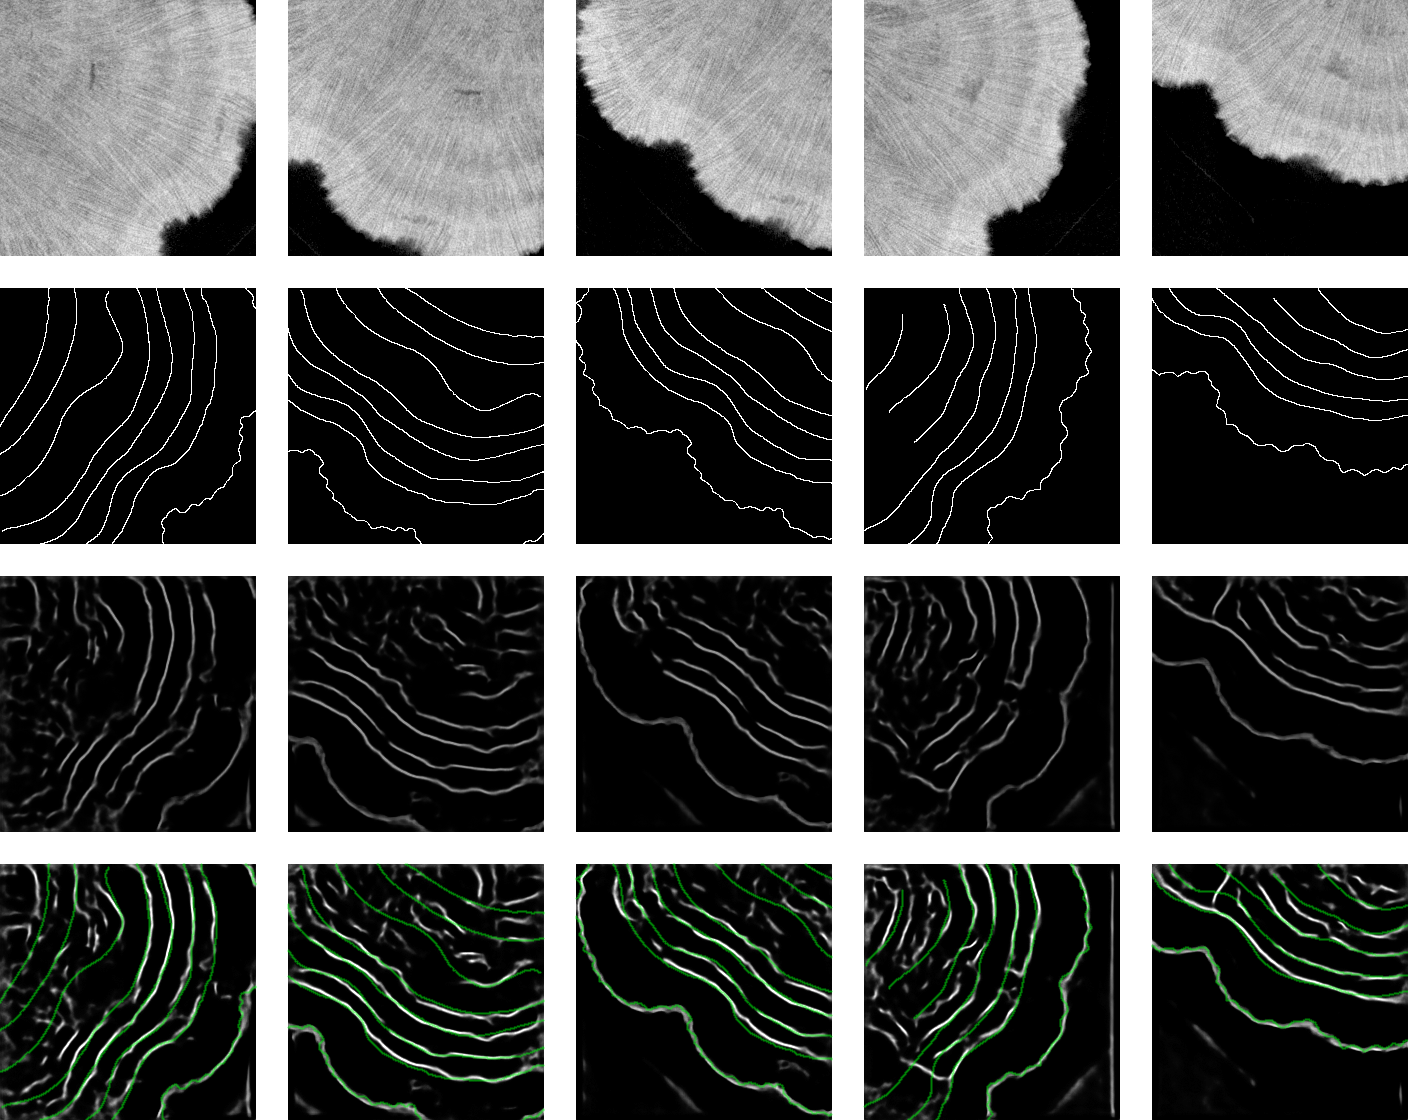
\includegraphics[width=1\textwidth]{images/initial-outputs.png}
    \caption{Good and bad results placeholder.}
    \label{fig:goodbad}
\end{figure}

The initial results achieved by the baseline model can be discussed further in order to gain a better understanding of the strengths and weaknesses of the model. The loss and accuracy curves are shown in Figure \ref{fig:basetrainacc} and example boundary predictions of both high and low ``quality'' are shown in Figure \ref{fig:goodbad}. Their quality is assessed both via the accuracy metric achieved and via visual inspection. Looking at Figure \ref{fig:basetrainacc}, it can be see that the accuracy achieved on the validation set is noticeably lower than the accuracy achieved on the training set. This unusual behaviour may be due to the validation set containing ``easier'' examples in which the annual banding is more obvious. Although the validation set may contain ... selection of easier ...

\subsection{Hyperparameter optimisation}

As discussed in Chapter \ref{chap:technical}, the performance achieved by deep neural networks is known to depend critically on the identification of a good set of hyperparameters~\cite{hyperparam, goodhyperparam}. In this project, a manual form of grid search was used to discover the optimal set of hyperparameter configurations. In this technique, all hyperparameters are fixed and only a single hyperparameter is varied at a time. Although this may not be the most efficient approach, it enables a better understanding of the model to be gained.

Due to the time constraints of the project, it would not be possible to perform an exhaustive search of all possible hyperparameter configurations. Thus, the primary aim of this chapter is not to achieve the best performance possible, but instead to evaluate which hyperparameters affect the performance most and reason as to why this is the case.

\subsubsection{Learning Rate}

Of all the hyperparameters relevant to deep learning models, the optimisation of the learning rate often has the biggest impact on the performance of a model~\cite{bengio2012practical}. The selection of a learning rate too large can cause an optimisation algorithm to take a step ``over'' minima causing the loss to inadvertently increase rather than decrease. The selection of a learning rate too small can also hinder performance as the optimisation algorithm may become permanently stuck in a suboptimal local minimum~\cite{goodfellow}.

Since it is usually not possible to calculate an optimal learning rate a priori~\cite{neuralbook}, some form of trial and error is required. A reasonable range of values to experiment with are given by Bengio in~\cite{bengio2012practical} and will be used as the basis of the values experimented with in this section. Bengio specifies a learning rate within the range of $10^{-6}$ to $1$ and recommends

NEED TO EITHER RENAME ACCURACY TO ERROR OR MAKE ACC LIKE (MAX POSSIBLE ERROR - VALUE) / MAX POSSIBLE ERROR

Maybe smooth previous graph on first page.

\begin{figure}[!t]
    \begin{subfigure}[b]{0.49\textwidth}
        \centering
        \begin{tikzpicture}[scale=0.9]
            \begin{axis}[
                height=\axisdefaultheight,
                ylabel=\small{Accuracy (pixels)},
                xlabel=\small{Epochs},
                grid=major,
                legend pos=north east,
                legend cell align=left,
                legend style={fill=white, fill opacity=0.8, draw=none,text opacity=1}]
                \addplot[magenta, mark=x] table [x=xs, y=lr00001_vacc, col sep=comma] {csv/lr.csv};
                \addlegendentry{\small{0.00001}}
                \addplot[darkgray, mark=x] table [x=xs, y=lr00005_vacc, col sep=comma] {csv/lr.csv};
                \addlegendentry{\small{0.00005}}
                \addplot[blue, mark=x] table [x=xs, y=lr0001_vacc, col sep=comma] {csv/lr.csv};
                \addlegendentry{\small{0.0001}}
                \addplot[orange, mark=x] table [x=xs, y=lr0005_vacc, col sep=comma] {csv/lr.csv};
                \addlegendentry{\small{0.0005}}
            \end{axis}
        \end{tikzpicture}
        \caption{Validaiton Accuracy}
    \end{subfigure}
    \hfill
    \begin{subfigure}[b]{0.49\textwidth}
        \centering
        \begin{tikzpicture}[scale=0.9]
            \begin{axis}[
                height=\axisdefaultheight,
                ylabel=\small{Accuracy (pixels)},
                xlabel=\small{Epochs},
                grid=major,
                legend pos=north east,
                legend cell align=left,
                legend style={fill=white, fill opacity=0.8, draw=none,text opacity=1}]
                \addplot[blue, mark=x] table [x=xs, y=ta, col sep=comma] {csv/base.csv};
                \addlegendentry{\small{Train Accuracy}}
                \addplot[magenta, mark=x] table [x=xs, y=va, col sep=comma] {csv/base.csv};
                \addlegendentry{\small{Val Accuracy}}
            \end{axis}
        \end{tikzpicture}
        \caption{Loss curve}
    \end{subfigure}
    \caption{Learning rate loss and accuracy plots. Apart from the learning rate, the same initial hyperparameters outlined in Table \ref{tab:initialhyperparams} were used once again.}
    \label{fig:lrplot}
\end{figure}

\subsubsection{Batch Size}

\subsubsection{Optimisation Algorithms}

Said in tech bg that I experimented with diff optimisers so need to add comparisons to SGD etc.

Look at the momentum values of adam? play around a little?

\subsubsection{Loss Functions}

\begin{figure}[t]
    \includegraphics[width=\textwidth, height=0.6\textwidth]{example-image-a}
    \caption{Focal loss examples vs cross-entropy loss examples.}
    \label{fig:lossfunctiondiff}
\end{figure}

Focal loss and other loss functions? to combat class imbalance

Look at the alpha and gamma values of focal loss? play around with them a little. look at the table in the original paper that says when you should use what.

\subsubsection{Dropout}

REMEMBER TO TRY AND UNDERSTAND WHY WHAT EVER HAPPENS IS THE CASE AND BACK IT UP ALL THROUGHOUT

vary from 0.1 to 0.9? same with spatial

\subsubsection{Spatial Dropout}

Need to talk about dropout? maybe only mention it in evaluation?
Spatial drop out better for fully conv? \url{https://arxiv.org/pdf/1411.4280.pdf}

% From Keras docs I think
% This version performs the same function as Dropout, however it drops
% entire 2D feature maps instead of individual elements. If adjacent pixels
% within feature maps are strongly correlated (as is normally the case in
% early convolution layers) then regular dropout will not regularize the
% activations and will otherwise just result in an effective learning rate
% decrease. In this case, SpatialDropout2D will help promote independence
% between feature maps and should be used instead.

\subsubsection{Kernel Sizes}

\subsubsection{L2 Regularization}

\subsection{Resolution}

\subsection{Augmentation}
\label{sec:evalaugmentation}

\subsubsection{No Augmentation}

\subsubsection{Augmentation Ranges}

\subsection{Ablation Studies}

comparison of convtranspose to upsample and then conv.

remove the relu at the end of the implementation?

Maybe visualise ablations with a graph showing each ablation with accuracy achieved or something? like in that paper. or a table?

\section{Three Dimensional Experimentation}

\subsection{Hyperparameter optimisation}

Due to the time constraints of the project, far fewer hyperparameters were optimised for the three dimensional architectures.

\subsection{Augmentation}

\subsection{Alternative Modified Architectures}

Varying numbers of output channels in Conv3D layers as you said youd experiment with this.

\subsection{Fully Three Dimensional Architecture}

\subsubsection{Data}

Lack of data. Was not consistently labelled. Show adjacent slices. Proves how hard it is to label images.

\section{Cross-validation}
\label{sec:evalcrossval}

\subsection{Train/test Splits}

\section{Final Results}

\begin{figure}[!p]
    \centering
    \includegraphics[width=\textwidth, height=1.45\textwidth]{example-image-b}
    \caption{A full page of final results achieved.}
    \label{fig:finalresults}
\end{figure}

\section{Comparisons with Other Architectures}

Compare SegNet, U-Net, pix2pix. Maybe find somewhere to put in the pix2pix generation for fun? If not don't worry. Do mention pix2pix using different backbones or whatever its called and why you think it didnt perform well.

\section{Critical Evaluation}

\subsection{Boundary Extraction}

\subsubsection{Labelling}

\subsubsection{Lack of Data}

very hard for a non expert to label.

\subsection{Accuracy Metric}

Can't tell which boundary it should be looking for. a completely white image would produce 100\% accuracy but the skeletonization makes the amount of white pixels low.

Maybe show concrete examples of where it falls down? images shifted to the right so that one boundary is roughly where another should be? images that have many white lines that are even perpendicular to the right labels should still produce a pretty low score?

\subsection{Calcification Rate Estimation}

\section{Comparisons with Existing Techniques}

Erica sent a paper a while ago that used a computer program to calculate the calcification rate  \url{https://www.geosociety.org/datarepository/2015/2015015.pdf} check the email from her with subject DeCarlo Paper

% {\bf A topic-specific chapter, of roughly $15$ pages} 
% \vspace{1cm} 

% \noindent
% This chapter is intended to evaluate what you did.  The content is highly 
% topic-specific, but for many projects will have flavours of the following:

% \begin{enumerate}
% \item functional  testing, including analysis and explanation of failure 
%       cases,
% \item behavioural testing, often including analysis of any results that 
%       draw some form of conclusion wrt. the aims and objectives,
%       and
% \item evaluation of options and decisions within the project, and/or a
%       comparison with alternatives.
% \end{enumerate}

% \noindent
% This chapter often acts to differentiate project quality: even if the work
% completed is of a high technical quality, critical yet objective evaluation 
% and comparison of the outcomes is crucial.  In essence, the reader wants to
% learn something, so the worst examples amount to simple statements of fact 
% (e.g., ``graph X shows the result is Y''); the best examples are analytical 
% and exploratory (e.g., ``graph X shows the result is Y, which means Z; this 
% contradicts [1], which may be because I use a different assumption'').  As 
% such, both positive {\em and} negative outcomes are valid {\em if} presented 
% in a suitable manner.